\documentclass[runningheads]{llncs}

% ---------------------------------------------------------------
% Include basic ECCV package

% TODO REVIEW: Insert your submission number below by replacing '*****'
% TODO FINAL: Comment out the following line for the camera-ready version
\usepackage[review,year=2026,ID=5364]{eccv}
% TODO FINAL: Un-comment the following line for the camera-ready version
%\usepackage{eccv}

% ---------------------------------------------------------------
% Other packages 

\usepackage{eccvabbrv}
\usepackage{graphicx}
\usepackage{booktabs}
\usepackage{amsmath,amssymb}
\usepackage{algorithm}
\usepackage{algorithmic}
\usepackage{multirow}
\usepackage{subcaption}
\usepackage{xcolor}
\usepackage{placeins}
\usepackage{float}
\usepackage{tikz}
\usetikzlibrary{arrows.meta,positioning,fit,backgrounds,calc,shapes.geometric}

% The "axessiblity" package can be found at: https://ctan.org/pkg/axessibility?lang=en
\usepackage[accsupp]{axessibility}

% ---------------------------------------------------------------
% Hyperref package
% TODO FINAL: Comment out the following line for the camera-ready version
\usepackage[pagebackref,breaklinks,colorlinks,citecolor=eccvblue]{hyperref}
% TODO FINAL: Un-comment the following line for the camera-ready version
%\usepackage{hyperref}
\usepackage[capitalize]{cleveref}

% Support for ORCID icon
\usepackage{orcidlink}

% Note: \eg, \ie, \etal are already defined by eccvabbrv

\begin{document}

% ---------------------------------------------------------------
\title{UrbanAlign: Post-hoc Semantic Calibration for VLM-Human Preference Alignment}

\titlerunning{UrbanAlign}

\author{Anonymous ECCV 2026 Submission}
\authorrunning{Anonymous}
\institute{Anonymous Institution}

\maketitle

% ===============================================================
% ABSTRACT
% ===============================================================
\begin{abstract}
Vision-language models (VLMs) can describe urban scenes in rich detail, yet consistently fail to produce reliable human preference labels in domain-specific tasks such as safety assessment and aesthetic evaluation.
The standard fix, fine-tuning or RLHF, requires large-scale annotations and model retraining.
We ask a different question: \emph{can a frozen VLM be aligned with human preferences without modifying any weights?}
Our key insight is that VLMs are strong concept extractors but poor decision calibrators.
We propose a three-stage post-hoc pipeline that exploits this asymmetry: (i)~interpretable evaluation dimensions are automatically mined from consensus exemplars; (ii)~an Observer--Debater--Judge chain extracts robust concept scores from the frozen VLM; and (iii)~locally-weighted ridge regression on a hybrid manifold calibrates these scores to human ratings.
Applied as \textbf{UrbanAlign} on Place Pulse~2.0, the framework reaches 72.2\% accuracy ($\kappa{=}0.45$) across six perception categories, outperforming all baselines by +11.0\,pp and zero-shot VLM by +15.5\,pp, with full interpretability and zero weight modification.

\keywords{Human Preference Alignment \and Post-hoc Concept Bottleneck \and Vision-Language Model \and Urban Perception}
\end{abstract}


% ===============================================================
% 1  INTRODUCTION
% ===============================================================
\section{Introduction}
\label{sec:intro}

Large vision-language models (VLMs) excel at describing visual scenes but consistently fail to produce reliable preference labels for domain-specific tasks.
This \emph{VLM--human preference alignment gap} appears across domains, from urban perception~\cite{zhang2025genai,mushkani2025dovlms} to aesthetic quality~\cite{murray2012ava,wu2024qalign}, and the standard remedy is model adaptation: fine-tuning, LoRA, or RLHF~\cite{ouyang2022training}, all of which modify model weights and require domain-specific training data and non-trivial compute.
We ask a different question: \emph{can a frozen VLM be aligned with human preferences in a new domain, without modifying any model weights?}

The key observation is that VLMs are already strong \emph{concept extractors} but poor \emph{decision calibrators}~\cite{zhang2025genai,mushkani2025dovlms}: they can identify rich visual elements in a scene (e.g., building facades, vegetation, and street infrastructure), yet their mapping from these features to discrete comparison labels is poorly aligned with human judgement boundaries (\cref{fig:comparison}).
This mirrors the finding of Concept Bottleneck Models (CBMs)~\cite{koh2020concept} that routing predictions through interpretable concept scores and then a calibrated linear layer dramatically outperforms end-to-end classification.
Such a bottleneck can be retrofitted \emph{post-hoc} onto any frozen backbone~\cite{yuksekgonul2023posthoc}, and recent work further shows that concepts can be discovered directly from VLMs without manual labels~\cite{oikarinen2023labelfree,yang2023language}.

A na\"{i}ve alternative is to prompt the VLM as a single-shot scorer, but this suffers from well-documented biases: position effects, anchoring, and inconsistent self-evaluation~\cite{wu2024qalign,liu2024pairs}.
When asked to compare two scenes directly, a single VLM call conflates perception and judgement: the model must simultaneously identify relevant visual cues, weigh their relative importance, and produce a discrete label, all within a single forward pass.
This end-to-end compression discards the structured reasoning that human raters implicitly perform when evaluating complex, multi-dimensional scenes.
Multi-agent debate protocols decompose complex judgements into complementary reasoning steps and have been shown to mitigate such biases through structured disagreement~\cite{du2024improving,wang2023selfconsistency}, yet these techniques have primarily targeted factual reasoning and text generation; their potential for domain-specific visual preference alignment remains unexplored.

This principle is operationalised as a pipeline that keeps the VLM entirely frozen, with three tightly coupled stages (\cref{fig:framework}):
\textbf{(i)}~\emph{concept mining}, where interpretable evaluation dimensions are discovered by the VLM from consensus exemplars;
\textbf{(ii)}~\emph{structured scoring}, where an Observer--Debater--Judge multi-agent chain extracts robust continuous concept scores from the frozen VLM;
\textbf{(iii)}~\emph{geometric calibration}, where locally-weighted ridge regression~\cite{cleveland1979robust} on a hybrid visual--semantic manifold aligns concept scores to human ratings.
An end-to-end optimization loop unifies these stages, automatically selecting the dimension set that maximises calibrated accuracy via temperature-scheduled trials.
We instantiate this framework as \textbf{UrbanAlign} on Place Pulse~2.0~\cite{salesses2013collaborative}, a large-scale pairwise comparison dataset covering six categories of urban perception, where subjective judgements~\cite{wilson1982broken,jacobs1961death} defy the feature-to-label mappings of existing approaches~\cite{dubey2016deep,naik2014streetscore}.
UrbanAlign substantially outperforms both supervised baselines and zero-shot VLM scoring across all six categories, with full dimension-level interpretability and zero model-weight modification, demonstrating that a frozen VLM already contains sufficient perceptual knowledge for human-aligned urban assessment.

\smallskip\noindent\textbf{Contributions.}
\begin{enumerate}
\item \textbf{End-to-end concept mining.} We design a loop that automatically discovers interpretable evaluation dimensions from consensus exemplars and refines them via a temperature-scheduled search, forming a concept bottleneck for perception prediction.
\item \textbf{Multi-agent structured scoring.} We introduce an Observer--Debater--Judge deliberation chain that extracts robust continuous concept scores from a frozen VLM, reducing single-agent bias through structured disagreement.
\item \textbf{Local geometric calibration.} We propose locally-weighted ridge regression on a hybrid visual--semantic manifold that calibrates concept scores against human ratings with per-sample interpretability.
\end{enumerate}


% ---------------------------------------------------------------
% Figure 1: Method comparison (three-pipeline conceptual diagram)
% ---------------------------------------------------------------
\begin{figure}[!ht]
\centering
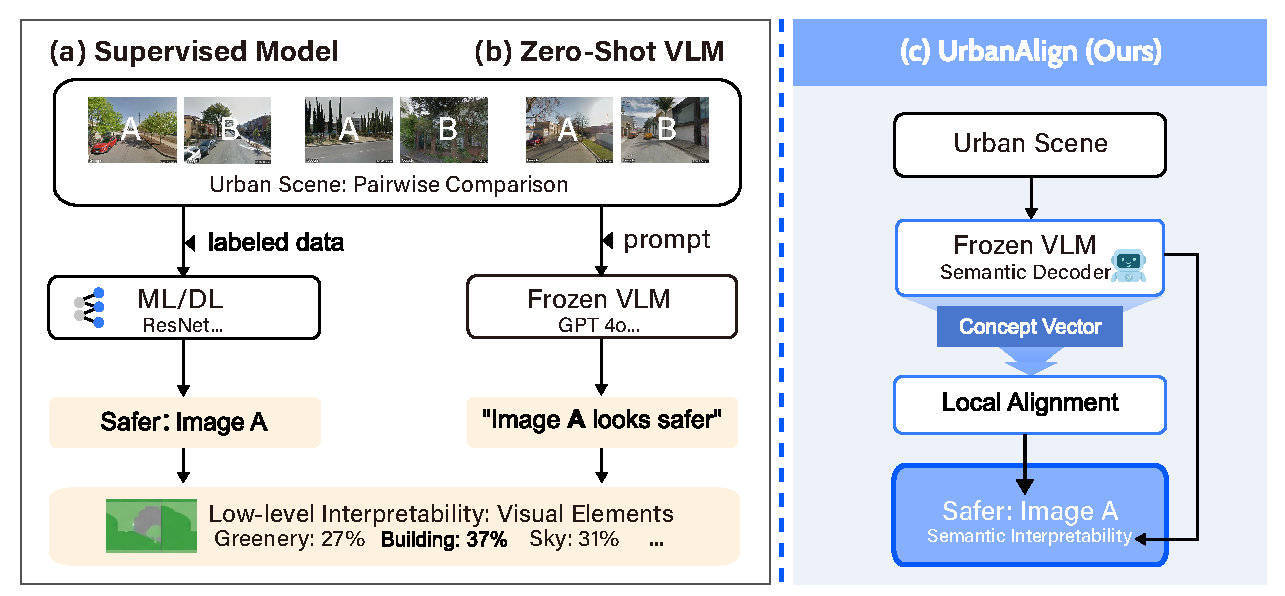
\includegraphics[width=\textwidth]{fig_comparison.pdf}
\caption{Three approaches to urban perception: \textbf{(a)}~supervised baselines (e.g., Siamese networks, segmentation regression) require labelled data and lack interpretable intermediates; \textbf{(b)}~zero-shot VLM prompting is training-free but produces opaque, uncalibrated judgements; \textbf{(c)}~UrbanAlign routes predictions through VLM-discovered semantic dimensions for interpretable, locally calibrated comparison.}
\label{fig:comparison}
\end{figure}

% ===============================================================
% 2  RELATED WORK
% ===============================================================
\section{Related Work}
\label{sec:related}

\noindent\textbf{Urban perception and preference data.}
\textcolor{red}{Pairwise comparison has a long history in psychometrics~\cite{thurstone1927law,bradley1952rank}.}
Place Pulse collects over one million pairwise comparisons of street-view images across six perceptual dimensions~\cite{salesses2013collaborative}.
Siamese networks~\cite{dubey2016deep}, multi-task learning~\cite{zhang2018measuring}, and continuous score regression~\cite{naik2014streetscore} have been trained on these labels, but map directly from pixels to abstract percepts without interpretable mid-level representations.
Cross-cultural evaluations further show that such models transfer poorly to non-Western cities~\cite{pp2chinese2025}, motivating cost-effective local calibration rather than large-scale re-annotation.
Pairwise preference datasets now extend to 10-dimension urban perception~\cite{quintana2025specs} and photographic aesthetics~\cite{murray2012ava}, \textcolor{red}{paralleling the learning-to-rank paradigm~\cite{joachims2002optimizing},} yet the resulting models remain black-box rankers.
Foundation models have been used to generate synthetic training corpora~\cite{ye2022zerogen,meng2023tuning}, but these operate on unimodal text with discrete labels and do not address the multi-dimensional, subjective nature of visual preference.
UrbanAlign instead synthesises \emph{visual} pairwise data via structured dimension scoring and post-hoc geometric calibration, requiring no weight modification.

\smallskip\noindent\textbf{VLM-based scoring and multi-agent reasoning.}
Systematic evaluation reveals that VLMs capture broad perceptual trends but oversimplify multi-dimensional human judgements~\cite{zhang2025genai}; benchmarking on urban perception confirms stronger alignment on objective properties (\eg, building density) than subjective ones (\eg, safety, boringness)~\cite{mushkani2025dovlms}.
Contrastive pretraining on satellite imagery~\cite{yan2024urbanclip} and zero-shot urban function inference~\cite{huang2024zeroshot} further demonstrate both the power and limits of VLMs for urban tasks; these studies position VLMs as end-to-end classifiers, whereas we reposition them as \emph{structured semantic decoders} whose outputs require post-hoc calibration.
Pairwise evaluation aligns better with human opinions than pointwise scoring~\cite{wu2024qalign,liu2024pairs}, yet single-shot scoring still suffers from position effects and anchoring biases.
Self-consistency sampling~\cite{wang2023selfconsistency} and multi-agent debate~\cite{du2024improving,liang2024encouraging,liu2025dmad} mitigate these issues for factual QA and mathematical reasoning, but applying structured deliberation to continuous visual scoring with domain-specific semantics remains unexplored.
UrbanAlign bridges this gap with an Observer--Debater--Judge chain that separates observation, argumentation, and judgement into distinct reasoning stages for pairwise dimension scoring.

\smallskip\noindent\textbf{\textcolor{red}{VLM preference alignment.}}
\textcolor{red}{Recent VLM alignment methods can be grouped by whether they modify model weights.
RLHF-based approaches train reward models and fine-tune the VLM via policy optimisation~\cite{ouyang2022training}; extensions augment this pipeline with factual grounding~\cite{sun2023factually} and vision-guided reinforcement that eliminates human annotation entirely~\cite{zhan2025visionr1}.
Robust visual reward models leverage auxiliary textual preference data to improve reward quality under scarce visual annotations~\cite{wang2024rovrm}, while implicit preference mining from user-generated content broadens the training signal beyond curated labels~\cite{tan2025implicit}.
All these methods require modifying VLM weights.
A parallel line calibrates VLM confidence post-hoc via semantic perturbation at the token level~\cite{zhao2025calibration}, but targets per-query confidence rather than domain-specific preference alignment.
UrbanAlign occupies a distinct position: it requires \emph{zero weight modification}, instead routing predictions through an external concept bottleneck with local geometric calibration---combining the interpretability of CBMs with the locality of retrieval-augmented prediction.}

\smallskip\noindent\textbf{Concept bottleneck models and post-hoc calibration.}
\textcolor{red}{Modern neural networks are known to be poorly calibrated~\cite{guo2017calibration}; temperature scaling and Platt scaling partially address this, but domain-specific preference alignment requires richer structural remedies.}
Concept Bottleneck Models (CBMs) route predictions through interpretable concept scores, enabling human-auditable reasoning and concept-level intervention~\cite{koh2020concept}.
Post-hoc retrofitting onto frozen backbones~\cite{yuksekgonul2023posthoc} and automated concept discovery from VLMs~\cite{oikarinen2023labelfree,yang2023language} eliminate manual concept engineering, making CBMs applicable without task-specific annotation of concept labels.
Our semantic dimensions serve as an analogous interpretable bottleneck, but operate \emph{externally} on VLM-synthesised data rather than as an internal network layer~\cite{srivastava2024vlgcbm,liu2025hybridcbm}: the VLM generates continuous concept scores, and a separate calibration step maps them to human-aligned predictions.

The calibration mechanism draws on locally-weighted regression~\cite{cleveland1979robust,atkeson1997locally,ruppert1994multivariate} and can be viewed as a visual analogue of retrieval-augmented generation (RAG)~\cite{lewis2020retrieval}: for each query pair, the system retrieves the $K$ most similar reference pairs from the hybrid manifold and locally fits a calibration function, adapting dimension weights to the manifold neighbourhood.
Unlike global linear probes or fixed concept weights, this local fitting allows the relative importance of dimensions to vary smoothly across the perceptual manifold, capturing the context-dependent nature of human preference.


% ===============================================================
% 3  METHOD
% ===============================================================
\newpage
\section{Method}
\label{sec:method}

% ---------------------------------------------------------------
% Figure 2: Framework overview
% ---------------------------------------------------------------
\begin{figure*}[t]
\centering
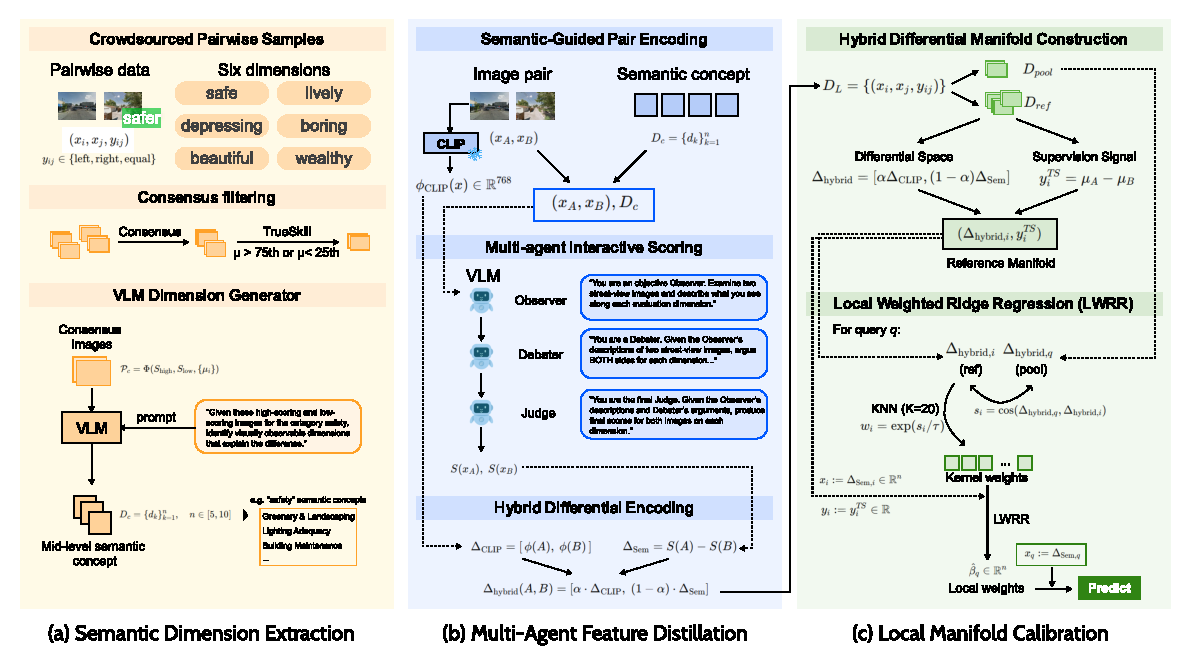
\includegraphics[width=\textwidth]{fig_framework.pdf}
\caption{UrbanAlign framework. Stage~1 mines semantic dimensions from consensus exemplars; Stage~2 distils dimension scores via Observer--Debater--Judge; Stage~3 calibrates via LWRR on the hybrid differential manifold. $\mathcal{D}_{\mathrm{ref}} \cap \mathcal{D}_{\mathrm{val}} \cap \mathcal{D}_{\mathrm{test}} = \varnothing$.}
\label{fig:framework}
\end{figure*}

\subsection{Problem Formulation}
\label{sec:formulation}

Given an urban image set $\mathcal{X}{=}\{x_1,\ldots,x_N\}$ and a perception category $d$ (\eg, wealthy), we aim to predict human pairwise preferences:
\begin{equation}
y_{ij} =
\begin{cases}
\text{left}  & \text{if } x_i \succ x_j \text{ on dimension } d,\\
\text{right} & \text{if } x_i \prec x_j,\\
\text{equal} & \text{if } x_i \approx x_j.
\end{cases}
\label{eq:pairwise}
\end{equation}
The labelled pool $\mathcal{D}_{L}{=}\{(x_i,x_j,y_{ij})\}$ contains crowdsourced pairwise comparisons (from Place Pulse~2.0).
We split $\mathcal{D}_{L}$ into a \emph{reference set} $\mathcal{D}_{\mathrm{ref}}$ (for LWRR calibration), a \emph{validation set} $\mathcal{D}_{\mathrm{val}}$ (for dimension and hyperparameter search), and a \emph{test set} $\mathcal{D}_{\mathrm{test}}$ (for final evaluation), with strict isolation: $\mathcal{D}_{\mathrm{ref}} \cap \mathcal{D}_{\mathrm{val}} \cap \mathcal{D}_{\mathrm{test}} = \varnothing$.

\noindent\textbf{Notation.}
$\phi{:}\,\mathcal{X}{\to}\mathbb{R}^{768}$ denotes a pre-trained CLIP encoder (ViT-L/14)~\cite{radford2021learning}.
TrueSkill~\cite{herbrich2006trueskill} converts pairwise comparisons to continuous ratings $\mu_i$ per image.

% ---------------------------------------------------------------
\subsection{Framework Overview}
\label{sec:overview}

The pipeline consists of three stages unified by an end-to-end optimization loop (\cref{fig:framework}).
\emph{Concept mining} (\cref{sec:stage1}) discovers interpretable evaluation dimensions from a handful of consensus exemplars and optimises them via a temperature-scheduled search.
\emph{Multi-agent structured scoring} (\cref{sec:stage2}) extracts continuous dimension scores from a frozen VLM through Observer--Debater--Judge deliberation, producing hybrid visual--semantic feature vectors.
\emph{Local manifold calibration} (\cref{sec:stage3}) aligns these scores to human ratings via locally-weighted ridge regression on the hybrid differential manifold.
Data isolation ($\mathcal{D}_{\mathrm{ref}} \cap \mathcal{D}_{\mathrm{val}} \cap \mathcal{D}_{\mathrm{test}} = \varnothing$) ensures that calibration, validation, and evaluation data never overlap.

% ---------------------------------------------------------------
\subsection{Concept Mining and Dimension Optimization (\cref{fig:framework}a)}
\label{sec:stage1}

\noindent\textbf{Motivation.}
Instead of asking a VLM ``Which image looks more wealthy?'' (a poorly calibrated end-to-end query), we first decompose the abstract percept into interpretable, continuously scorable sub-dimensions.
This is analogous to defining the concept set in a CBM~\cite{koh2020concept}: the dimensions form an interpretable bottleneck through which all subsequent predictions must pass.

\smallskip\noindent\textbf{TrueSkill consensus sampling.}
We convert pairwise comparisons to continuous scores via TrueSkill~\cite{herbrich2006trueskill}.
We sample \emph{high-consensus} ($\mu{>}\tau_{h},\;\sigma{<}\sigma_{\mathrm{med}}$) and \emph{low-consensus} ($\mu{<}\tau_{l},\;\sigma{<}\sigma_{\mathrm{med}}$) exemplars, where $\tau_{h}$ and $\tau_{l}$ are the 75th and 25th percentiles.
A small set per group forms the consensus set $\mathcal{S}_{\mathrm{consensus}}$.

\smallskip\noindent\textbf{Dimension extraction.}
A structured prompt presents the high/low exemplars with their TrueSkill scores and PCA-compressed CLIP embeddings.
The VLM outputs $n\in[5,10]$ dimensions in JSON, each containing a name, description, and high/low indicators \textcolor{red}{(exact schema and prompts in supplementary Section~D)}.
For the \emph{wealthy} category, the extracted dimensions are:
\emph{Fa\c{c}ade Quality}, \emph{Vegetation Maintenance}, \emph{Pavement Integrity}, \emph{Vehicle Quality}, \emph{Building Modernity}, \emph{Infrastructure Condition}, \emph{Street Cleanliness}, and \emph{Lighting Quality}.

These dimensions satisfy three requirements: \emph{visual observability} (scorable from street-view images), \emph{measurability} (1--10 continuous scale), and \emph{universality} (applicable across cities).

\smallskip\noindent\textbf{End-to-end dimension optimization.}
The dimensions discovered above depend on the VLM's sampling temperature and the particular consensus exemplars presented.
We close the loop with an automated search over dimension sets, optimising each perception category independently.
Let $\mathcal{D}_c^{(t)}$ denote the dimension set generated at trial $t$ for category $c$.
Each trial runs the full pipeline (dimension extraction $\to$ multi-agent scoring $\to$ LWRR calibration) on the held-out validation split $\mathcal{D}_{\mathrm{val}}$.
The per-category optimal set is:
\begin{equation}
\mathcal{D}_c^{*} = \arg\max_{t \in \{1,\ldots,T\}} \;\mathrm{Acc}_c\bigl(\text{LWRR}\bigl(\text{Score}(\mathcal{D}_{\mathrm{val}}^{c},\, \mathcal{D}_c^{(t)}),\, \mathcal{D}_{\mathrm{ref}}^{c}\bigr)\bigr).
\label{eq:e2e}
\end{equation}
The search proceeds in two phases:
\emph{Explore} (high $\tau_{\mathrm{gen}}$): diverse, independently generated dimension sets; each category accumulates its best.
\emph{Converge} (low $\tau_{\mathrm{gen}}$): per-category best dimensions are preserved except for 1--2 targeted replacements (\emph{mutation mode}), enabling local refinement.
Since categories may peak at different trials, the final output \emph{assembles} per-category optima: $\{\mathcal{D}_c^{*}\}_{c=1}^{C}$.

% ---------------------------------------------------------------
\subsection{Multi-Agent Structured Scoring (\cref{fig:framework}b)}
\label{sec:stage2}

\noindent\textbf{From classification to feature extraction.}
Rather than querying a VLM for a one-shot discrete label, we extract a \emph{hybrid feature vector}:
\begin{equation}
h(x) = [\phi_{\text{CLIP}}(x),\; S(x)],
\label{eq:hybrid}
\end{equation}
where $S(x)\in[1,10]^{n}$ is the vector of semantic dimension scores produced by the VLM, fusing low-level visual patterns with high-level domain semantics analogously to a post-hoc CBM~\cite{yuksekgonul2023posthoc}.

\smallskip\noindent\textbf{Observer--Debater--Judge deliberation.}
Inspired by multi-agent debate~\cite{du2024improving,liang2024encouraging} and self-consistency~\cite{wang2023selfconsistency}, we decompose reasoning into three sequentially chained agents:

\begin{itemize}
\item \textbf{Observer}: describes visually observable details per dimension, without judgement, thereby suppressing confirmation bias.
\item \textbf{Debater}: argues both for HIGH and LOW scores on each dimension, exploring opposing perspectives.
\item \textbf{Judge}: synthesises descriptions and arguments to produce final scores $S(x)\in[1,10]^{n}$.
\end{itemize}

\noindent\textbf{Variance reduction.}
The three-agent chain reduces dimension score variance from $\sigma_S^2$ to at most $\sigma_S^2/(1{+}2(1{-}\rho))$, where $\rho\in[0,1]$ is inter-agent correlation; when agents reason independently ($\rho{\to}0$), variance drops by up to $3\times$ (proof in supplementary Section~E).

\smallskip\noindent\textbf{Intensity-based winner determination.}
For each pair $(x_A, x_B)$, we also record the \emph{intensity}: $I{=}|S(x_A) - S(x_B)|$ summed across dimensions.
Pairs with intensity below a threshold $\sigma_I$ are labelled ``equal''; otherwise the VLM's predicted winner is retained.

% ---------------------------------------------------------------
\subsection{Local Manifold Calibration (\cref{fig:framework}c)}
\label{sec:stage3}

This stage is the core algorithmic contribution: a post-hoc calibration layer analogous to the linear predictor in a CBM~\cite{koh2020concept}, but \emph{locally adaptive} to account for heterogeneous perception patterns across the visual-semantic manifold.

\subsubsection{Hybrid Differential Space.}

CLIP, pre-trained on web-scale image-text pairs, provides strong general features but exhibits distribution shift on street-view scenes.
We augment it with semantic dimension scores to form the hybrid differential encoding:
\begin{equation}
\Delta_{\text{hybrid}}(A,B)=\bigl[\alpha\cdot\overline{\Delta}_{\text{CLIP}}(A,B),\;(1{-}\alpha)\cdot\overline{\Delta}_{\text{Sem}}(A,B)\bigr],
\label{eq:hybrid_diff}
\end{equation}
where $\overline{\Delta}_{\text{CLIP}}$ uses L2-normalised CLIP embeddings, $\Delta_{\text{Sem}}{=}S(A){-}S(B)$ is normalised to $[0,1]$ by dividing by 10, and $\alpha\in[0,1]$ balances visual and semantic components.

\subsubsection{LWRR Algorithm.}
Our calibration extends locally-weighted regression~\cite{cleveland1979robust,atkeson1997locally,ruppert1994multivariate} to the hybrid differential space defined above.

\noindent\textbf{Step~1: Build reference manifold.}
From $\mathcal{D}_{\mathrm{ref}}$, compute hybrid differential vectors and TrueSkill score differences $y_i^{\text{TS}}{=}\mu_A{-}\mu_B$.
Mirror augmentation doubles the reference set: for each $(A,B,y)$, add $(B,A,-y)$.

\noindent\textbf{Step~2: Neighbourhood search.}
For query $\Delta_q^{\mathrm{hybrid}} \in \mathcal{D}_{\mathrm{test}}$, compute cosine similarities to all reference points and select the $K$ nearest neighbours $\mathcal{N}_K$.

\noindent\textbf{Step~3: Kernel weighting.}
$w_i=\exp(s_i/\tau)$ for $i\in\mathcal{N}_K$, where $s_i$ is cosine similarity and $\tau$ is kernel bandwidth.

\noindent\textbf{Step~4: Local ridge regression.}
Solve for local dimension weights:
\begin{equation}
\hat{\mathbf{w}} = \arg\min_{\mathbf{w}} \sum_{i\in\mathcal{N}_K} w_i\bigl(y_i^{\text{TS}}-\mathbf{w}^{\!\top}\Delta_{\text{Sem},i}\bigr)^{2} + \lambda\|\mathbf{w}\|^{2},
\label{eq:lwrr}
\end{equation}
with closed-form solution $\hat{\mathbf{w}}=(X^{\!\top}WX+\lambda I)^{-1}X^{\!\top}Wy$, where $W{=}\mathrm{diag}(w_1,\ldots,w_K)$ and $X$ stacks the semantic differentials.

\noindent\textbf{Step~5: Prediction.}
The calibrated score difference $\hat{\delta}_q = \hat{\mathbf{w}}^{\!\top}\Delta_{\text{Sem}}^{q}$; a local goodness-of-fit statistic provides per-prediction interpretability by measuring how much TrueSkill variance is explainable by the mid-level dimensions in each neighbourhood.

\noindent\textbf{Step~6: Statistical re-inference.}
\begin{equation}
\hat{y} =
\begin{cases}
\text{equal} & \text{if } |\hat{\delta}|<\varepsilon \text{ or } c_{\mathrm{eq}}>\theta, \\
\text{left}  & \text{if } \hat{\delta}>0, \\
\text{right} & \text{otherwise},
\end{cases}
\label{eq:reinfer}
\end{equation}
where $\varepsilon$ is a score-difference threshold and $c_{\mathrm{eq}}{=}|\{i\in\mathcal{N}_K: l_i{=}\text{equal}\}|/K$ measures local equal-consensus.

\begin{theorem}[Local Calibration Bound]\label{thm:calibration}
\textcolor{red}{(Adapted from classical locally-weighted regression~\cite{cleveland1979robust,caponnetto2007optimal} to the hybrid VLM-concept manifold.)}
Under the local model $y_i^{\mathrm{TS}} = w^{*\!}(q)^{\!\top} \Delta_{\mathrm{Sem},i} + \epsilon_i$ within $\mathcal{N}_K(q)$, with zero-mean noise of variance~$\sigma^2$, the LWRR estimator satisfies:
\begin{equation}
\mathbb{E}\bigl[\|\hat{w} - w^{*\!}(q)\|^2\bigr]
\;\leq\;
\frac{\sigma^2\,\mathrm{tr}(H_\lambda^{-1}X^{\!\top}W^2\!X\,H_\lambda^{-1})}{K}
\;+\;
\lambda^2\|w^{*}\|^2,
\label{eq:lwrr_bound}
\end{equation}
where $H_\lambda = X^{\!\top}\!W\!X + \lambda I$.
At optimal $\lambda^{*} \!=\! \sigma\sqrt{n/K}/\|w^{*}\|$, this simplifies to $O(\sigma\|w^{*}\|\sqrt{n/K})$.
\textcolor{red}{The key implication for our setting is that with $n{=}5$--$8$ concept dimensions and $K{=}20$ neighbours, the system is well-overdetermined ($K \gg n$), ensuring small estimation variance; in contrast, a global model incurs irreducible bias from manifold heterogeneity (supplementary Theorem~2).}
\emph{Proof in supplementary Section~E.}
\end{theorem}

\noindent \textcolor{red}{The following decomposition provides intuitive guidance for why each pipeline stage is necessary, though it is approximate rather than a formal bound:}
\begin{equation}
\mathrm{Acc} \;\approx\; \Phi\!\left(\frac{\|w^{*}\|\,\bar{\delta}}{\sqrt{\sigma_{\mathrm{LWRR}}^{2} + \sigma_{S}^{2}/\eta_{M}}}\right),
\label{eq:accuracy}
\end{equation}
where $\bar{\delta}$ is the mean signal strength (maximised by concept mining), $\sigma_S^2$ is dimension-score variance (reduced by multi-agent scoring with $\eta_M$-fold gain), and $\sigma_{\mathrm{LWRR}}^2$ is calibration error (minimised by LWRR).
\textcolor{red}{Each pipeline stage tightens a specific term: Stage~1 maximises $\bar{\delta}$, Stage~2 minimises $\sigma_S^2/\eta_M$, and Stage~3 minimises $\sigma_{\mathrm{LWRR}}^2$; a formal end-to-end bound is given in supplementary Corollary~2.}
Full pseudocode in supplementary Section~H; additional theory (local vs.\ global calibration, E2E convergence) in Section~E.


% ===============================================================
% 4  EXPERIMENTS
% ===============================================================
\section{Experiments and Results}
\label{sec:exp}

\subsection{Setup}

\noindent\textbf{Dataset.}
Place Pulse 2.0~\cite{salesses2013collaborative}: 110,688 street-view images from 56 cities with 1,169,078 pairwise comparisons across six perception categories (safety, lively, beautiful, wealthy, depressing, boring).
We retain all pairs with ${\geq}2$ independent human votes (449--1,412 per category).
Results span \textbf{all six categories}; detailed ablation on \emph{wealthy}.

\smallskip\noindent\textbf{Data protocol.}
Each category is partitioned into $\mathcal{D}_{\mathrm{ref}}$ (60\%), $\mathcal{D}_{\mathrm{val}}$ (20\%), and $\mathcal{D}_{\mathrm{test}}$ (20\%); $\mathcal{D}_{\mathrm{ref}} \cap \mathcal{D}_{\mathrm{val}} \cap \mathcal{D}_{\mathrm{test}} = \varnothing$ (stratified split, seed\,=\,42).
$\mathcal{D}_{\mathrm{ref}}$ provides TrueSkill ratings for LWRR calibration; $\mathcal{D}_{\mathrm{val}}$ serves dimension search (\cref{eq:e2e}) and hyperparameter selection; $\mathcal{D}_{\mathrm{test}}$ is held out for final evaluation.
After excluding human ``equal'' labels, 83--260 test pairs per category remain.

\smallskip\noindent\textbf{Implementation.}
CLIP ViT-L/14 (768-d) for visual features; PCA to 8D for consensus prompts.
GPT-4o~\cite{openai2024gpt4o} as the default VLM\textcolor{red}{; backbone-agnostic design is verified with Qwen2.5-VL-72B~\cite{bai2025qwen25vl} (\cref{sec:sensitivity})}.
TrueSkill priors: $\mu{=}25$, $\sigma{=}8.33$, draw probability 0.10; 5 images per consensus group (10 total).
Stage~2: Observer $\tau{=}0.3$, Debater $\tau{=}0.5$, Judge $\tau{=}0.1$; single-shot modes $\tau{=}0.0$.
Stage~3 defaults: $K{=}20$, $\tau_{\mathrm{kernel}}{=}1.0$, $\lambda{=}1.0$, $\varepsilon{=}0.8$, $\theta{=}0.6$, $\alpha{=}0.3$.
E2E dimension search: $T{=}15$ trials with patience-based early stopping after 5 non-improving trials; explore phase $\tau_{\mathrm{gen}}{=}0.85{\to}1.0$, converge phase $\tau_{\mathrm{gen}}{=}0.7{\to}0.5$.
Total VLM cost: {\raise.17ex\hbox{$\scriptstyle\sim$}}\$68 for the experimental dataset (4,819 pairs, Mode~4)\textcolor{red}{; wall-clock time ${\sim}$2--4\,h with concurrent API access, no GPU required (supplementary Section~K)}.
The main results (\cref{tab:main}) use \emph{per-category} optimised hyperparameters from a combined random search ($N{=}50{,}000$ configurations on $\mathcal{D}_{\mathrm{val}}$; supplementary Section~C), as the optimal $K$ (10--50) and $\alpha$ (0.2--0.7) vary substantially across categories.

\smallskip\noindent\textbf{Baselines.}
\emph{ResNet-50 Siamese}: twin-tower on frozen ResNet-50 features~\cite{koch2015siamese};
\emph{CLIP Siamese}: same architecture on CLIP ViT-L/14 features;
\emph{Seg.\ + CLIP Regression}: SegFormer segmentation proportions + PCA-reduced CLIP, classified by Gradient Boosting~\cite{chen2018deeplabv3plus};
\emph{Zero-shot VLM}: GPT-4o with forced binary prompt (no dimensions or multi-agent reasoning).
All supervised baselines use the reference split with mirror augmentation.


% ---------------------------------------------------------------
\subsection{Main Results}

\Cref{tab:main} and \cref{fig:comparison} present the main comparison; \cref{fig:qualitative} provides per-pair qualitative evidence.
Key findings:

(1)~UrbanAlign achieves 72.2\% average accuracy ($\kappa{=}0.45$), outperforming the strongest same-feature control (Global Ridge on $\Delta_{\mathrm{sem}}$: 61.2\%) by \textbf{+11.0\,pp} and zero-shot VLM (56.7\%) by +15.5\,pp, with 81.6\% ($\kappa{=}0.64$) on \emph{safety}; the gap over same-feature controls confirms that local calibration---not feature quality alone---is the key differentiator.
(2)~LWRR calibration provides +16.3\,pp average boost (55.9\%$\to$72.2\%), with the largest effect on \emph{boring} (+31.3\,pp) and \emph{depressing} (+25.3\,pp), where raw predictions are near chance.
(3)~The gap between \emph{safety} (81.6\%) and \emph{boring} (70.2\%) reflects perceptual grounding: safety correlates with concrete cues~\cite{wilson1982broken,jeffery1971cpted}, while boringness depends on subtler absence-of-stimulation signals.
\textcolor{red}{(4)~Human split-half agreement on Place Pulse ranges from 78--87\% across categories (supplementary Section~L); on \emph{safety}, UrbanAlign matches this ceiling (81.8\% vs.\ 81.6\%), while on other categories an 9--18\,pp gap remains.
Bootstrap 95\% CIs for UrbanAlign accuracy are $\pm$5--10\,pp, reflecting moderate test-set sizes (83--260 pairs per category); all lower bounds exceed the 56.7\% zero-shot baseline.}

\vspace{-2mm}
\begin{table}[H]
\centering
\caption{Comparison on Place Pulse 2.0 across all six perception categories. All values reported as excl-equal\,(incl-equal). UrbanAlign outperforms all baselines including same-feature controls (72.2\% vs.\ 61.2\% best baseline).}
\label{tab:main}
\resizebox{\columnwidth}{!}{
\begin{tabular}{l cc cc cc}
\toprule
 & \multicolumn{2}{c}{Safety} & \multicolumn{2}{c}{Beautiful} & \multicolumn{2}{c}{Lively} \\
\cmidrule(lr){2-3} \cmidrule(lr){4-5} \cmidrule(lr){6-7}
Method & Acc.(\%) & $\kappa$ & Acc.(\%) & $\kappa$ & Acc.(\%) & $\kappa$ \\
\midrule
ResNet50 Siamese~\cite{koch2015siamese} & 54.8\,(54.0) & 0.16\,(0.18) & 58.6\,(56.0) & 0.18\,(0.19) & 45.7\,(42.5) & $-$0.07\,($-$0.06) \\
CLIP Siamese~\cite{radford2021learning} & 66.7\,(64.4) & 0.34\,(0.31) & 61.4\,(57.3) & 0.23\,(0.20) & 48.2\,(44.8) & $-$0.01\,($-$0.01) \\
Seg.\ Regression~\cite{chen2018deeplabv3plus} & 61.9\,(59.8) & 0.25\,(0.23) & 57.1\,(53.3) & 0.15\,(0.13) & 51.9\,(48.3) & 0.04\,(0.04) \\
GPT-4o zero-shot~\cite{openai2024gpt4o} & 61.9\,(59.8) & 0.23\,(0.21) & 62.9\,(58.7) & 0.25\,(0.21) & 49.4\,(46.0) & 0.01\,(0.01) \\
\addlinespace[2pt]
\textcolor{red}{BT Logistic~\cite{bradley1952rank}}\textsuperscript{\dag} & 65.5\,(63.2) & 0.31\,(0.29) & 58.6\,(54.7) & 0.17\,(0.15) & 56.8\,(52.9) & 0.17\,(0.15) \\
Global Ridge\textsuperscript{\dag} & 66.7\,(64.4) & 0.33\,(0.31) & 61.4\,(57.3) & 0.22\,(0.19) & 58.0\,(54.0) & 0.19\,(0.17) \\
\midrule
UrbanAlign (Ours) & \textbf{81.6}\,(76.9) & \textbf{0.64}\,(0.57) & \textbf{69.8}\,(66.7) & \textbf{0.38}\,(0.35) & \textbf{69.4}\,(65.4) & \textbf{0.40}\,(0.36) \\
\midrule
 & \multicolumn{2}{c}{Wealthy} & \multicolumn{2}{c}{Boring} & \multicolumn{2}{c}{Depressing} \\
\cmidrule(lr){2-3} \cmidrule(lr){4-5} \cmidrule(lr){6-7}
Method & Acc.(\%) & $\kappa$ & Acc.(\%) & $\kappa$ & Acc.(\%) & $\kappa$ \\
\midrule
ResNet50 Siamese~\cite{koch2015siamese} & 47.0\,(44.8) & 0.01\,(0.00) & 48.7\,(45.0) & $-$0.00\,($-$0.02) & 53.3\,(50.0) & 0.06\,(0.05) \\
CLIP Siamese~\cite{radford2021learning} & 57.8\,(55.2) & 0.19\,(0.17) & 50.0\,(47.5) & 0.06\,(0.07) & 58.7\,(55.0) & 0.19\,(0.16) \\
Seg.\ Regression~\cite{chen2018deeplabv3plus} & 61.5\,(58.6) & 0.26\,(0.23) & 62.2\,(57.5) & 0.22\,(0.19) & 54.7\,(52.5) & 0.09\,(0.11) \\
GPT-4o zero-shot~\cite{openai2024gpt4o} & 60.2\,(57.5) & 0.21\,(0.19) & 48.7\,(45.0) & 0.06\,(0.05) & 57.3\,(53.8) & 0.14\,(0.12) \\
\addlinespace[2pt]
\textcolor{red}{BT Logistic~\cite{bradley1952rank}}\textsuperscript{\dag} & 68.7\,(65.5) & 0.38\,(0.35) & 50.0\,(46.3) & 0.01\,(0.01) & 58.7\,(55.0) & 0.17\,(0.15) \\
Global Ridge\textsuperscript{\dag} & 69.9\,(66.7) & 0.40\,(0.37) & 54.1\,(50.0) & 0.10\,(0.08) & 57.3\,(53.8) & 0.15\,(0.13) \\
\midrule
UrbanAlign (Ours) & \textbf{74.0}\,(71.2) & \textbf{0.48}\,(0.44) & \textbf{70.2}\,(68.8) & \textbf{0.41}\,(0.40) & \textbf{68.2}\,(62.5) & \textbf{0.37}\,(0.31) \\
\bottomrule
\end{tabular}}
\\[4pt]
\footnotesize{\textsuperscript{*}Excl-equal excludes ``equal'' labels; model ``equal'' predictions count as errors. $\mathcal{D}_{\mathrm{test}}$: 83--260 pairs/cat. Same GPT-4o backbone for UrbanAlign and zero-shot. \textsuperscript{\dag}Trained on UrbanAlign's $\Delta_{\mathrm{sem}}$ with $\mathcal{D}_{\mathrm{ref}}$ labels.}
\end{table}

% ---------------------------------------------------------------
\subsection{Dimension-Level Discriminability}

\Cref{tab:dim_disc} shows discriminability varies substantially across categories: \emph{wealthy} (avg.\ 68.0\%) and \emph{safety} (64.7\%) are highest, while \emph{depressing} (42.1\%) is weakest, suggesting that ``depressingness'' is harder to decompose into visually scorable sub-dimensions.
For \emph{wealthy}, \emph{Fa\c{c}ade Quality}, \emph{Street Cleanliness}, and \emph{Pavement Integrity} all reach 71.2\%, consistent with broken-windows theory~\cite{wilson1982broken}.
LWRR's aggregate accuracy (74.0\%) exceeds any single dimension, validating the multi-dimensional concept bottleneck: the local weight combination captures complementary information that no individual dimension alone provides.

\smallskip\noindent\textbf{Why does the pipeline outperform end-to-end alternatives?}
Accuracy (\cref{eq:accuracy}) decomposes into three terms, each targeted by a stage: concept mining maximises signal strength~$\bar{\delta}$ (avg.\ 54.7\%; \cref{tab:dim_disc}); multi-agent scoring reduces $\sigma_{S}^{2}$; LWRR minimises calibration error by fitting weights \emph{locally}.
The hybrid space ($\alpha{=}0.3$) is critical: CLIP provides neighbourhood structure while semantic scores supply domain signals; global ridge on hybrid features (57.8\%) underperforms semantic-only (61.2\%), confirming this role separation.

\smallskip\noindent\textbf{Interpretability and qualitative analysis.}
For a high-confidence pair, LWRR weights reveal Building Modernity ($w{=}2.30$), Vegetation Maintenance ($w{=}1.72$), and Street Cleanliness ($w{=}1.35$) as top contributors---directly actionable for urban planners.
\Cref{fig:qualitative} visualises per-pair reasoning across all six categories; ``Corrected'' cases show LWRR overturning incorrect raw predictions via local re-weighting.

\begin{table}[t]
\centering
\caption{Per-dimension discriminative power (Mode~4). ``Power'' = fraction (\%) of test pairs where the score difference on that single dimension correctly predicts the human winner (50\% = chance). $n$ = test pairs; ``avg'' = mean power across all dimensions.}
\label{tab:dim_disc}
\resizebox{\columnwidth}{!}{
\begin{tabular}{lc|lc|lc}
\toprule
\multicolumn{2}{c|}{\textbf{Safety} ($n{=}283$, avg 64.7\%)} & \multicolumn{2}{c|}{\textbf{Beautiful} ($n{=}125$, avg 56.7\%)} & \multicolumn{2}{c}{\textbf{Lively} ($n{=}259$, avg 53.0\%)} \\
Dimension & Power & Dimension & Power & Dimension & Power \\
\midrule
Greenery \& Landscaping & 71.2 & Greenery \& Nat.\ Elem. & 64.4 & Human Presence & 59.6 \\
Lighting Adequacy & 71.2 & Color Coordination & 62.2 & Building Diversity & 57.7 \\
Building Maintenance & 69.2 & Pedestrian Amenities & 55.6 & Street Furniture & 57.7 \\
Pedestrian Infrastructure & 65.4 & Street Cleanliness & 55.6 & Color \& Lighting & 53.8 \\
Street Activity & 57.7 & Architectural Coherence & 55.6 & Commercial Activity & 53.8 \\
Visibility Clarity & 53.8 & Visual Complexity & 46.7 & Public Art \& Signage & 46.2 \\
 & & & & Vegetation \& Greenery & 42.3 \\
\midrule
\multicolumn{2}{c|}{\textbf{Wealthy} ($n{=}117$, avg 68.0\%)} & \multicolumn{2}{c|}{\textbf{Boring} ($n{=}91$, avg 43.8\%)} & \multicolumn{2}{c}{\textbf{Depressing} ($n{=}95$, avg 42.1\%)} \\
Dimension & Power & Dimension & Power & Dimension & Power \\
\midrule
Fa\c{c}ade Quality & 71.2 & Activity Presence & 52.1 & Street Cleanliness & 47.9 \\
Street Cleanliness & 71.2 & Color Vibrancy & 50.0 & Visual Clutter & 45.8 \\
Pavement Integrity & 71.2 & Street Furn.\ Presence & 47.9 & Fa\c{c}ade Condition & 43.8 \\
Vegetation Maintenance & 69.2 & Architectural Diversity & 43.8 & Lighting Quality & 39.6 \\
Lighting Quality & 67.3 & Visual Complexity & 39.6 & Greenery Presence & 33.3 \\
Infrastructure Condition & 67.3 & Spatial Enclosure & 37.5 & & \\
Vehicle Quality & 65.4 & Vegetation Variety & 35.4 & & \\
Building Modernity & 61.5 & & & & \\
\bottomrule
\end{tabular}}
\\[2pt]
\footnotesize{5--10 dims/category; E2E loop explores alternatives over 15 trials.}
\end{table}

\begin{figure*}[p]
\centering
\includegraphics[width=\textwidth]{fig_qualitative.pdf}
\caption{Qualitative examples across six perception categories. \textbf{A}~denotes the human-selected winner (green border). \emph{Centre chart}: per-dimension concept scores for image~A (\textcolor{green!60!black}{green}) and image~B (\textcolor{blue!70!black}{blue}) on the left half, and LWRR contribution towards~A on the right half\textcolor{red}{; the $y$-axis lists dimension names and bar length represents each dimension's contribution to $\hat{\delta}_q$ (\cref{eq:lwrr})}; positive LWRR bars support~A, negative bars support~B. The summary line reports the raw score comparison and calibrated LWRR delta; ``Corrected'' marks cases where calibration overturns an incorrect raw prediction. \emph{Right chart}: baseline confidence bars (\textcolor{orange}{orange}~=~conf.\,A, \textcolor{violet}{purple}~=~conf.\,B, \textcolor{gray}{grey}~=~equal); UrbanAlign is shown in bold.}
\label{fig:qualitative}
\end{figure*}
\clearpage\setlength{\parskip}{0pt}\raggedbottom%
% ---------------------------------------------------------------
\refstepcounter{subsection}\label{sec:ablation}%
\noindent{\normalsize\bfseries\boldmath 4.4\quad Ablation Study}\par\nobreak\vspace{8pt}%
\noindent We ablate four scoring modes crossing two factors: input context (single-image vs.\ pairwise) and reasoning protocol (single-shot vs.\ multi-agent), yielding Modes~1--4 (\cref{tab:factorial}).

\smallskip\noindent\textbf{Component analysis.}
Zero-shot VLM scoring (C3, 56.7\%, \cref{tab:main}) lacks interpretable intermediates.
Structured dimension scoring (Mode~2 raw, 55.4\%) achieves comparable accuracy while creating a concept bottleneck that decomposes each prediction into 5--8 interpretable dimension scores.
Multi-agent deliberation (Mode~4 raw, 55.9\%) reduces dimension-score variance, producing more consistent calibration inputs.
LWRR then leverages this low-variance bottleneck for +16.3\,pp (72.2\%): locally-adapted weights capture complementary information inaccessible to holistic scoring.
E2E dimension search confirms default dimensions are near-optimal (69.3\% vs.\ 72.2\%; Section~\ref{sec:sensitivity}).

\textcolor{red}{\noindent\textbf{Note on dimensions and hyperparameters.}
\Cref{tab:main} reports results using the \emph{original} Stage-1 dimensions with per-category \emph{optimised calibration hyperparameters} (from a combined random search on $\mathcal{D}_{\mathrm{val}}$; supplementary Section~C).
The E2E dimension search (\cref{eq:e2e}) optimises only the \emph{dimension set} while holding calibration hyperparameters at defaults, achieving 69.3\%.
These two optimisation axes are complementary and have not yet been combined, leaving room for further improvement.}

\noindent\textbf{$\mathbf{2{\times}2}$ factorial design.}
\textcolor{red}{We isolate pairwise context and multi-agent reasoning via a $2{\times}2$ factorial (\cref{tab:factorial}, averaged across all six categories, post-LWRR; per-category breakdown in supplementary Table~13).
\textbf{Multi-agent reasoning} consistently improves accuracy: +5.0\,pp on single-image inputs and +20.3\,pp on pairwise inputs on average.
\textbf{Pairwise context} alone yields only a marginal +1.0\,pp (Mode~1$\to$2), as without deliberation dual inputs introduce noise in some categories (\eg, \emph{wealthy}: $-$13.2\,pp, \emph{lively}: $-$7.4\,pp); however, it strongly \emph{amplifies} multi-agent reasoning (+16.3\,pp, Mode~3$\to$4), as comparative anchors fuel constructive debate.
The two factors interact \textbf{synergistically}: Mode~4 exceeds Mode~1 by +21.3\,pp on average, far exceeding the sum of individual effects (+6.0\,pp), with consistent synergy across all six categories (supplementary Table~13).}

\noindent\textbf{LWRR calibration gain.}
\Cref{tab:vrm_gain_main}: LWRR yields +16.3\,pp average (55.9\%$\to$72.2\%), with the largest effect on \emph{boring} (+31.3\,pp) and \emph{depressing} (+25.3\,pp), categories where raw predictions are near chance and benefit most from locally-adapted dimension weighting.
Full per-mode breakdown in supplementary Section~G.
\begingroup\setlength{\intextsep}{4mm}%
\begin{table}[H]
\centering
\caption{\textcolor{red}{$2{\times}2$ factorial averaged across all six categories (accuracy\%\,/\,$\kappa$, post-LWRR). Per-category results in supplementary Table~13.}}
\label{tab:factorial}
\small
\begin{tabular}{l|cc|c}
\toprule
 & Single-Shot & Multi-Agent & Multi-Agent Gain \\
\midrule
\textcolor{red}{Single-Image} & \textcolor{red}{50.9\,/\,0.08} & \textcolor{red}{55.9\,/\,0.18} & \textcolor{red}{+5.0} \\
\textcolor{red}{Pairwise}     & \textcolor{red}{51.9\,/\,0.10} & \textcolor{red}{\textbf{72.2}\,/\,\textbf{0.45}} & \textcolor{red}{+20.3} \\
\midrule
\textcolor{red}{Pairwise Gain} & \textcolor{red}{+1.0} & \textcolor{red}{+16.3} & --- \\
\bottomrule
\end{tabular}
\end{table}\endgroup
\begingroup\setlength{\intextsep}{4mm}%
\begin{table}[H]
\centering
\caption{LWRR calibration gain (Mode~4, excl.\ ``equal''). All six categories improve; avg.\ +16.3\,pp.}
\label{tab:vrm_gain_main}
\small
\begin{tabular}{lcccccc|c}
\toprule
 & Safety & Beaut. & Lively & Wealthy & Boring & Depress. & Avg \\
\midrule
Raw Acc.\ (\%)     & 68.4 & 63.9 & 58.5 & 62.9 & 38.9 & 42.9 & 55.9 \\
Aligned Acc.\ (\%) & 81.6 & 69.8 & 69.4 & 74.0 & 70.2 & 68.2 & 72.2 \\
$\Delta$ (pp)      & \textbf{+13.3} & \textbf{+5.9} & \textbf{+10.9} & \textbf{+11.1} & \textbf{+31.3} & \textbf{+25.3} & \textbf{+16.3} \\
\midrule
Raw $\kappa$       & 0.38 & 0.29 & 0.17 & 0.26 & $-$0.22 & $-$0.13 & 0.13 \\
Aligned $\kappa$   & 0.64 & 0.38 & 0.40 & 0.48 & 0.41 & 0.37 & 0.45 \\
\midrule
$n$ (test pairs)   & 260 & 115 & 238 & 107 & 83 & 87 & --- \\
\bottomrule
\end{tabular}
\end{table}\endgroup

% ---------------------------------------------------------------
\subsection{Sensitivity Analysis}
\label{sec:sensitivity}

Full grids in supplementary Section~C.
$K_{\max}$ is most sensitive (+4.3\,pp; $K{=}20$ best on average); $\alpha{=}0.3$ (70\% semantic) is optimal but per-category optima differ; $\tau_{\mathrm{kernel}}$ and $\lambda_{\mathrm{ridge}}$ have limited effect ($<$2.5\,pp); scoring thresholds $\varepsilon$ and $\theta$ are robust.
The E2E dimension loop (\cref{eq:e2e}, 12/15 trials) yields 69.3\% via per-category assembly; the main pipeline (72.2\%) uses optimised calibration hyperparameters with original dimensions (supplementary Sections~C,~F).

\smallskip\noindent\textbf{Backbone generalization.}
\textcolor{red}{Replacing GPT-4o with Qwen2.5-VL-72B~\cite{bai2025qwen25vl} and re-optimising Stage~3 hyperparameters yields 72.5\% ($\kappa{=}0.45$), matching GPT-4o within 0.3\,pp across all categories (supplementary Section~J), confirming backbone-agnostic design.}

% ===============================================================
% 5  CONCLUSION
% ===============================================================
\section{Conclusion}
\label{sec:conclusion}

We presented \textbf{UrbanAlign}, a post-hoc calibration framework that transforms frozen VLMs from unreliable annotators (56.7\%) into structured perception decoders (72.2\%, $\kappa{=}0.45$) via interpretable semantic dimensions and locally-adaptive geometric calibration, without modifying any model weights.
Its three stages---concept mining~\cite{koh2020concept}, multi-agent scoring~\cite{du2024improving}, and locally-weighted ridge regression on a hybrid manifold---are mutually reinforcing: on Place Pulse~2.0 the combination surpasses all baselines, with the largest gains on near-chance categories (\emph{boring}: +31.3\,pp, \emph{depressing}: +25.3\,pp), while the per-pair LWRR weights remain directly interpretable.

\smallskip\noindent\textbf{Limitations and future work.}
Urban perception labels can encode societal biases; UrbanAlign's interpretable dimension weights expose but do not eliminate such biases, and deployment for planning decisions should be paired with equity-aware review.
Natural next steps include extending to cross-cultural settings~\cite{pp2chinese2025,quintana2025specs} where demographic factors modulate perception, and generalising to other pairwise-preference domains such as aesthetic quality.
\textcolor{red}{Code and data splits will be released upon acceptance.}
Extended discussion is in supplementary Section~K.

% ---- Bibliography ----
\bibliographystyle{splncs04}
\bibliography{main}
\end{document}
